\documentclass[aspectratio=169]{beamer}

% Theme and Color Setup
\usetheme{Madrid}
\usecolortheme{whale}
\useinnertheme{rectangles}
\useoutertheme{miniframes}

% Additional Packages
\usepackage[utf8]{inputenc}
\usepackage[T1]{fontenc}
\usepackage{graphicx}
\usepackage{booktabs}
\usepackage{listings}
\usepackage{amsmath}
\usepackage{amssymb}
\usepackage{xcolor}
\usepackage{tikz}
\usepackage{pgfplots}
\pgfplotsset{compat=1.18}
\usetikzlibrary{positioning}
\usepackage{hyperref}

% Custom Colors
\definecolor{myblue}{RGB}{31, 73, 125}
\definecolor{mygray}{RGB}{100, 100, 100}
\definecolor{mygreen}{RGB}{0, 128, 0}
\definecolor{myorange}{RGB}{230, 126, 34}
\definecolor{mycodebackground}{RGB}{245, 245, 245}

% Set Theme Colors
\setbeamercolor{structure}{fg=myblue}
\setbeamercolor{frametitle}{fg=white, bg=myblue}
\setbeamercolor{title}{fg=myblue}
\setbeamercolor{section in toc}{fg=myblue}
\setbeamercolor{item projected}{fg=white, bg=myblue}
\setbeamercolor{block title}{bg=myblue!20, fg=myblue}
\setbeamercolor{block body}{bg=myblue!10}
\setbeamercolor{alerted text}{fg=myorange}

% Set Fonts
\setbeamerfont{title}{size=\Large, series=\bfseries}
\setbeamerfont{frametitle}{size=\large, series=\bfseries}
\setbeamerfont{caption}{size=\small}
\setbeamerfont{footnote}{size=\tiny}

% Code Listing Style
\lstdefinestyle{customcode}{
  backgroundcolor=\color{mycodebackground},
  basicstyle=\footnotesize\ttfamily,
  breakatwhitespace=false,
  breaklines=true,
  commentstyle=\color{mygreen}\itshape,
  keywordstyle=\color{blue}\bfseries,
  stringstyle=\color{myorange},
  numbers=left,
  numbersep=8pt,
  numberstyle=\tiny\color{mygray},
  frame=single,
  framesep=5pt,
  rulecolor=\color{mygray},
  showspaces=false,
  showstringspaces=false,
  showtabs=false,
  tabsize=2,
  captionpos=b
}
\lstset{style=customcode}

% Footer and Navigation Setup
\setbeamertemplate{footline}{
  \leavevmode%
  \hbox{%
  \begin{beamercolorbox}[wd=.3\paperwidth,ht=2.25ex,dp=1ex,center]{author in head/foot}%
    \usebeamerfont{author in head/foot}\insertshortauthor
  \end{beamercolorbox}%
  \begin{beamercolorbox}[wd=.5\paperwidth,ht=2.25ex,dp=1ex,center]{title in head/foot}%
    \usebeamerfont{title in head/foot}\insertshorttitle
  \end{beamercolorbox}%
  \begin{beamercolorbox}[wd=.2\paperwidth,ht=2.25ex,dp=1ex,center]{date in head/foot}%
    \usebeamerfont{date in head/foot}
    \insertframenumber{} / \inserttotalframenumber
  \end{beamercolorbox}}%
  \vskip0pt%
}

% Turn off navigation symbols
\setbeamertemplate{navigation symbols}{}

% Title Page Information
\title[Academic Template]{Week 14: Course Review and Assessment}
\author[J. Smith]{John Smith, Ph.D.}
\institute[University Name]{
  Department of Computer Science\\
  University Name\\
  \vspace{0.3cm}
  Email: email@university.edu\\
  Website: www.university.edu
}
\date{\today}

% Document Start
\begin{document}

\frame{\titlepage}

\begin{frame}[fragile]
    \frametitle{Course Review Introduction}
    \begin{block}{Overview of Course Objectives}
        This course has provided a comprehensive understanding of the fundamental concepts of data processing at scale, particularly within the domains of big data and machine learning. Our objectives have included:
    \end{block}
\end{frame}

\begin{frame}[fragile]
    \frametitle{Course Review Objectives}
    \begin{enumerate}
        \item \textbf{Understanding Data Characteristics}:
        \begin{itemize}
            \item Different types of data (structured, unstructured, semi-structured).
            \item The volume, velocity, variety, and veracity of big data (the 4Vs).
        \end{itemize}

        \item \textbf{Data Processing Frameworks}:
        \begin{itemize}
            \item Introduction to tools and frameworks for processing big data, such as Hadoop and Apache Spark.
            \item Learning the importance and application of distributed systems.
        \end{itemize}

        \item \textbf{Data Analysis Techniques}:
        \begin{itemize}
            \item Exploring various methodologies like MapReduce for efficient data processing.
            \item Application of machine learning algorithms to extract insights from large datasets.
        \end{itemize}

        \item \textbf{Real-world Applications}:
        \begin{itemize}
            \item Discussing the role of data processing in industries such as finance, healthcare, and marketing.
        \end{itemize}
    \end{enumerate}
\end{frame}

\begin{frame}[fragile]
    \frametitle{Importance of Data Processing at Scale}
    Data processing at scale is essential in today's data-driven world for several reasons:
    \begin{itemize}
        \item \textbf{Efficiency}:
        Traditional methods of processing data can be slow and ineffective. Scalable systems allow us to process data quickly and efficiently.
        \begin{itemize}
            \item \textit{Example}: A retail company analyzing millions of transactions to improve stock management.
        \end{itemize}
        
        \item \textbf{Cost-Effectiveness}:
        Handling large datasets often requires robust systems that operate economically and reduce overhead costs.
        
        \item \textbf{Actionable Insights}:
        Rapid data processing enables businesses to draw actionable insights more quickly than ever.
        \begin{itemize}
            \item \textit{Illustration}: A social media platform processing user interactions to tailor advertisements in real-time.
        \end{itemize}

        \item \textbf{Scalability}:
        As data grows, scalability ensures systems can grow in power and capacity without performance degradation.
    \end{itemize}
\end{frame}

\begin{frame}[fragile]
    \frametitle{Key Points & Conclusion}
    \begin{block}{Key Points to Emphasize}
        \begin{itemize}
            \item The 4Vs of Big Data are foundational for analyzing large datasets.
            \item Distributed computing frameworks like Hadoop and Spark are pivotal in processing data effectively.
            \item Real-world examples highlight the practical implications of data processing at scale.
        \end{itemize}
    \end{block}

    \begin{block}{Conclusion}
        By reviewing the key course objectives, we prepare to appreciate the vital role of scalable data processing in technology and business landscapes.
    \end{block}
\end{frame}

\begin{frame}[fragile]
    \frametitle{Key Concepts in Data Processing - Overview}
    \begin{itemize}
        \item Understanding core principles: 
            \begin{itemize}
                \item Distributed Computing
                \item Parallel Processing
                \item MapReduce Methodology
            \end{itemize}
        \item Importance of these concepts for efficient data management and analysis.
    \end{itemize}
\end{frame}

\begin{frame}[fragile]
    \frametitle{Key Concept 1: Distributed Computing}
    \begin{block}{Definition}
        A model where a single task is divided across multiple networked computers (nodes) that work together to process data.
    \end{block}
    \begin{itemize}
        \item \textbf{Example:} 
            Analyzing customer purchase data from multiple stores where each store’s computer processes its own data concurrently.
        \item \textbf{Key Point:} 
            Improves scalability and performance by utilizing multiple resources efficiently.
    \end{itemize}
\end{frame}

\begin{frame}[fragile]
    \frametitle{Key Concept 2: Parallel Processing}
    \begin{block}{Definition}
        Simultaneous execution of multiple processes to enhance computational speed and efficiency.
    \end{block}
    \begin{itemize}
        \item \textbf{Example:} 
            Video rendering where each segment is processed on a separate core of a multi-core processor.
        \item \textbf{Key Point:} 
            Essential for tasks that can be subdivided, improving overall computational efficiency.
    \end{itemize}
\end{frame}

\begin{frame}[fragile]
    \frametitle{Key Concept 3: MapReduce Methodology}
    \begin{block}{Definition}
        A programming model for processing and generating large datasets with a parallel, distributed algorithm.
    \end{block}
    \begin{itemize}
        \item \textbf{Map Function:} 
            Processes input (key-value pairs) to produce intermediate key-value pairs.
        \item \textbf{Reduce Function:} 
            Aggregates intermediate key-value pairs to produce final output.
        \item \textbf{Example:} 
            Word counting where the map function emits <word, 1> and the reduce function sums occurrences.
        \item \textbf{Key Point:} 
            Allows for fault tolerance and data locality, vital for distributed system processing.
    \end{itemize}    
\end{frame}

\begin{frame}[fragile]
    \frametitle{Basic MapReduce Workflow Illustration}
    \begin{block}{Workflow Steps}
        \texttt{Input Data -> Map -> Intermediate Data -> Shuffle and Sort -> Reduce -> Final Output}
    \end{block}
    \begin{itemize}
        \item \textbf{Map:} Processes and emits key-value pairs.
        \item \textbf{Shuffle and Sort:} Organizes data by keys (automatic).
        \item \textbf{Reduce:} Combines values for each unique key to derive final results.
    \end{itemize}
\end{frame}

\begin{frame}[fragile]
    \frametitle{Industry-Standard Tools - Introduction}
    \begin{itemize}
        \item Importance of proficiency in industry-standard tools for data management, analysis, and processing.
        \item Overview of key tools:
            \begin{itemize}
                \item Programming languages: Python, R, SQL
                \item Frameworks: Apache Spark, Hadoop
            \end{itemize}
        \item Enhance technical skills and prepare for real-world data science applications.
    \end{itemize}
\end{frame}

\begin{frame}[fragile]
    \frametitle{Key Tools and Frameworks}
    \begin{enumerate}
        \item \textbf{Python}
            \begin{itemize}
                \item Versatile programming language for data analysis and machine learning.
                \item Example Libraries: Pandas, NumPy, Scikit-learn.
                \item \begin{lstlisting}[language=Python]
import pandas as pd
data = pd.read_csv('data.csv')
print(data.describe())
                \end{lstlisting}
            \end{itemize}

        \item \textbf{R}
            \begin{itemize}
                \item Primarily used for statistical analysis and data visualization.
                \item Key Features: extensive libraries and strong community support.
                \item \begin{lstlisting}[language=R]
data <- read.csv('data.csv')
summary(data)
                \end{lstlisting}
            \end{itemize}

        \item \textbf{SQL}
            \begin{itemize}
                \item Standard language for relational databases.
                \item Example Query: 
                \begin{lstlisting}[language=SQL]
SELECT name, age FROM users WHERE age > 30;
                \end{lstlisting}
            \end{itemize}
    \end{enumerate}
\end{frame}

\begin{frame}[fragile]
    \frametitle{Big Data Frameworks}
    \begin{enumerate}
        \item \textbf{Apache Spark}
            \begin{itemize}
                \item Open-source analytics engine designed for speed and sophisticated analytics.
                \item Key Component: Spark SQL for structured data processing.
            \end{itemize}

        \item \textbf{Hadoop}
            \begin{itemize}
                \item Framework for distributed processing of large data sets via MapReduce.
                \item Architecture: HDFS for storage and YARN for resource management.
                \item (Envision a simplified architecture diagram showing HDFS and YARN components with various data nodes.)
            \end{itemize}
    \end{enumerate}
\end{frame}

\begin{frame}[fragile]
    \frametitle{Evaluating Data Processing Methodologies - Introduction}
    Understanding the effectiveness of data processing methodologies is crucial in developing efficient systems for handling large datasets. 
    This slide outlines key criteria for evaluating these methodologies and offers practical applications to ensure clarity and relatability.
\end{frame}

\begin{frame}[fragile]
    \frametitle{Evaluating Data Processing Methodologies - Criteria for Evaluation}
    \begin{enumerate}
        \item \textbf{Efficiency}
        \begin{itemize}
            \item \textbf{Definition}: The speed at which data can be processed.
            \item \textbf{Example}: SQL excels in complex queries but may lag in real-time processing.
        \end{itemize}
        
        \item \textbf{Scalability}
        \begin{itemize}
            \item \textbf{Definition}: The ability to handle increasing volumes of data.
            \item \textbf{Example}: Apache Spark efficiently processes petabytes of data across distributed systems.
        \end{itemize}
        
        \item \textbf{Flexibility}
        \begin{itemize}
            \item \textbf{Definition}: The adaptability to various types of data.
            \item \textbf{Example}: Python integrates with various libraries like Pandas and Matplotlib.
        \end{itemize}
        
        \item \textbf{Cost-Effectiveness}
        \begin{itemize}
            \item \textbf{Definition}: The overall cost of implementation and maintenance.
            \item \textbf{Example}: Open-source frameworks like Apache Hadoop reduce costs compared to proprietary systems.
        \end{itemize}
        
        \item \textbf{Ease of Use}
        \begin{itemize}
            \item \textbf{Definition}: The user-friendliness of tools and methods.
            \item \textbf{Example}: R offers user-friendly syntax and extensive documentation.
        \end{itemize}
    \end{enumerate}
\end{frame}

\begin{frame}[fragile]
    \frametitle{Evaluating Data Processing Methodologies - Practical Applications}
    \begin{enumerate}
        \item \textbf{Example in E-Commerce}:
        \begin{itemize}
            \item \textbf{Scenario}: An online retailer uses Apache Spark for real-time customer data processing.
            \item \textbf{Criterion Application}:
            \begin{itemize}
                \item \textbf{Efficiency}: Spark's in-memory processing allows for fast analysis.
                \item \textbf{Scalability}: More nodes can be added as the customer base grows.
            \end{itemize}
        \end{itemize}
        
        \item \textbf{Example in Healthcare}:
        \begin{itemize}
            \item \textbf{Scenario}: A hospital employs SQL databases for patient data management and risk prediction.
            \item \textbf{Criterion Application}:
            \begin{itemize}
                \item \textbf{Flexibility}: SQL queries can adapt to new data types.
                \item \textbf{Cost-Effectiveness}: Utilizing existing infrastructure reduces costs.
            \end{itemize}
        \end{itemize}
    \end{enumerate}
\end{frame}

\begin{frame}[fragile]
    \frametitle{Evaluating Data Processing Methodologies - Key Points}
    \begin{itemize}
        \item A combination of these criteria allows for a holistic view of strengths and weaknesses.
        \item Choosing the right methodology based on specific organizational needs can significantly impact performance and effectiveness.
    \end{itemize}
    
    \begin{block}{Diagram (Conceptual Representation)}
        \textit{A flowchart illustrating the evaluation process should be included here, showcasing how to assess efficiency, scalability, flexibility, cost-effectiveness, and ease of use when selecting a data processing methodology.}
    \end{block}
    
    In summary, evaluating various data processing methodologies based on the outlined criteria can lead to improved data handling and increased organizational success.
\end{frame}

\begin{frame}[fragile]
    \frametitle{Designing Data Processing Workflows}
    \begin{block}{Overview}
        Designing data processing workflows is essential for efficiently managing large datasets and deriving actionable insights. This slide outlines the steps to create comprehensive workflows while emphasizing best practices.
    \end{block}
\end{frame}

\begin{frame}[fragile]
    \frametitle{Steps to Design and Execute Data Processing Workflows}
    \begin{enumerate}
        \item \textbf{Define Objectives:}
        \begin{itemize}
            \item Clarify Goals: Determine the purpose of data processing.
            \item Example: A retail company analyzes sales data to identify seasonal trends.
        \end{itemize}

        \item \textbf{Data Collection:}
        \begin{itemize}
            \item Identify Sources: Select relevant data sources like databases or APIs.
            \item Example: Gather customer transaction data from point-of-sale systems.
        \end{itemize}

        \item \textbf{Data Preparation:}
        \begin{itemize}
            \item Cleaning: Remove duplicates and fill in missing values.
            \item Transformation: Convert and aggregate data.
        \end{itemize}
    \end{enumerate}
\end{frame}

\begin{frame}[fragile]
    \frametitle{Data Preparation (continued) and Processing}
    \begin{block}{Code Snippet}
        \begin{lstlisting}[language=Python]
import pandas as pd
data = pd.read_csv('sales_data.csv')
data.drop_duplicates(inplace=True)
data.fillna(0, inplace=True)  # Fill missing values with 0
        \end{lstlisting}
    \end{block}

    \begin{enumerate}[resume]
        \item \textbf{Data Processing:}
        \begin{itemize}
            \item Select Methodologies: Choose data processing techniques.
            \item Example Application: Use Apache Spark for analyzing real-time web traffic data.
        \end{itemize}

        \item \textbf{Analysis and Visualization:}
        \begin{itemize}
            \item Generate Insights: Analyze processed data for meaningful outputs.
            \item Visualization Tools: Use Tableau or Matplotlib for effective storytelling.
        \end{itemize}
    \end{enumerate}
\end{frame}

\begin{frame}[fragile]
    \frametitle{Validation, Documentation, and Execution}
    \begin{enumerate}[resume]
        \item \textbf{Validation:}
        \begin{itemize}
            \item Verify Results: Conduct quality checks for accuracy.
            \item Feedback Loop: Implement continuous review mechanisms.
        \end{itemize}

        \item \textbf{Documentation:}
        \begin{itemize}
            \item Record the Workflow: Capture decisions and results for reference.
            \item Importance: Enables reproducibility and continuous improvement.
        \end{itemize}

        \item \textbf{Execution:}
        \begin{itemize}
            \item Deploy Workflows: Use Apache Airflow for automation.
            \item Monitoring: Set up alerts for failures or performance issues.
        \end{itemize}
    \end{enumerate}
\end{frame}

\begin{frame}[fragile]
    \frametitle{Best Practices}
    \begin{itemize}
        \item Iterate and Improve: Continuous improvement is vital.
        \item Collaborate \& Communicate: Regular engagement with stakeholders ensures alignment.
        \item Scalability \& Flexibility: Design adaptable workflows for growing data volumes.
    \end{itemize}
\end{frame}

\begin{frame}[fragile]
    \frametitle{Key Points to Emphasize}
    \begin{itemize}
        \item Clear Objectives are paramount for effective workflows.
        \item Data Quality must be maintained throughout.
        \item Leverage Automation Tools to manage complexity efficiently.
    \end{itemize}
\end{frame}

\begin{frame}[fragile]
    \frametitle{Collaboration and Communication}
    \begin{block}{Overview}
        In the context of data processing and analysis, effective collaboration and communication are essential skills. 
        Working in teams often enhances creativity and leads to better problem-solving.
        This slide focuses on the importance of teamwork, effective communication, and presenting technical findings in a collaborative environment.
    \end{block}
\end{frame}

\begin{frame}[fragile]
    \frametitle{Key Concepts - Teamwork}
    \begin{itemize}
        \item \textbf{Definition:} A collective effort where individuals contribute their skills and expertise towards a common goal.
        \item \textbf{Importance:} 
        \begin{itemize}
            \item \textit{Diverse Perspectives:} Members provide varied insights, enhancing decision-making.
            \item \textit{Shared Responsibilities:} Tasks can be allocated based on strengths, increasing efficiency.
        \end{itemize}
        \item \textbf{Example:} In a data science project:
        \begin{itemize}
            \item One member focuses on data cleaning.
            \item Another on analysis.
            \item A third on visualization, all crucial for successful outcomes.
        \end{itemize}
    \end{itemize}
\end{frame}

\begin{frame}[fragile]
    \frametitle{Key Concepts - Effective Communication}
    \begin{itemize}
        \item \textbf{Definition:} The ability to convey information clearly and effectively.
        \item \textbf{Importance:}
        \begin{itemize}
            \item \textit{Clarity:} Ensures all team members have a shared understanding of project goals and roles.
            \item \textit{Feedback:} Facilitates process improvement through constructive criticism.
        \end{itemize}
        \item \textbf{Example:} Use of data visualization tools (e.g., Tableau, Power BI) to communicate complex data findings to non-technical stakeholders.
    \end{itemize}
\end{frame}

\begin{frame}[fragile]
    \frametitle{Key Concepts - Presentation of Findings}
    \begin{itemize}
        \item \textbf{Definition:} Sharing outcomes of data analysis in an understandable format.
        \item \textbf{Importance:}
        \begin{itemize}
            \item \textit{Accessibility:} Technical insights must be conveyed accessibly to diverse audiences.
            \item \textit{Visualization:} Graphs, charts, and infographics make data more relatable.
        \end{itemize}
        \item \textbf{Example:} Presenting machine learning model predictions using visual aids to clarify trends and insights.
    \end{itemize}
\end{frame}

\begin{frame}[fragile]
    \frametitle{Key Points to Emphasize}
    \begin{itemize}
        \item \textbf{Collaboration is Crucial:} Foster an environment where team input is valued.
        \item \textbf{Communication Tools Matter:} Tools like Slack, Microsoft Teams, and project management software enhance coordination.
        \item \textbf{Mindful of Your Audience:} Tailor communication style to the audience's technical expertise.
        \item \textbf{Feedback Loop:} Establish mechanisms for regular feedback to adapt and improve team processes.
    \end{itemize}
\end{frame}

\begin{frame}[fragile]
    \frametitle{Diagram: Effective Communication Cycle}
    \begin{center}
        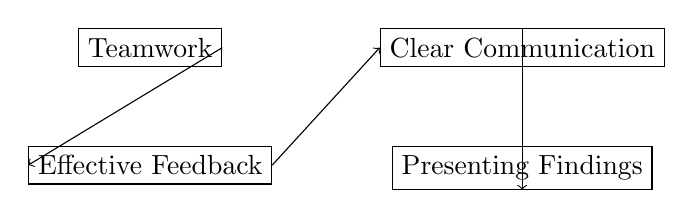
\begin{tikzpicture}
            \node (teamwork) [draw, rectangle] {Teamwork};
            \node (feedback) [draw, rectangle, below=1cm of teamwork] {Effective Feedback};
            \node (communication) [draw, rectangle, right=2cm of teamwork] {Clear Communication};
            \node (findings) [draw, rectangle, below=1cm of communication] {Presenting Findings};

            \path[->] (teamwork.east) edge (feedback.west);
            \path[->] (communication.north) edge (findings.south);
            \path[->] (feedback.east) edge (communication.west);
        \end{tikzpicture}
    \end{center}
\end{frame}

\begin{frame}[fragile]
    \frametitle{Conclusion}
    Incorporating teamwork and effective communication into data processing projects leads to better outcomes and a positive work environment. 
    Strong collaborative efforts can transform technical findings into actionable insights, driving innovation and progress.
\end{frame}

\begin{frame}[fragile]
    \frametitle{Data Governance and Ethics}
    \begin{block}{Overview}
        Review of ethical considerations and governance frameworks in data processing, supported by case studies.
    \end{block}
\end{frame}

\begin{frame}[fragile]
    \frametitle{Key Concepts}
    \begin{itemize}
        \item \textbf{Data Governance:} Overall management of data availability, usability, integrity, and security within an organization.
        \item \textbf{Ethics in Data Processing:} Responsible use of data respecting individual rights and societal values, emphasizing transparency, accountability, and fairness.
    \end{itemize}
\end{frame}

\begin{frame}[fragile]
    \frametitle{Importance of Data Governance and Ethics}
    \begin{enumerate}
        \item \textbf{Trust and Transparency:}
            \begin{itemize}
                \item Establish a culture of trust through transparent data use.
                \item Example: GDPR emphasizes transparency regarding personal data.
            \end{itemize}
        \item \textbf{Compliance with Laws:}
            \begin{itemize}
                \item Adhering to regulations protects organizations from legal issues.
                \item Example: HIPAA governs the use of health information in the U.S.
            \end{itemize}
        \item \textbf{Risk Management:}
            \begin{itemize}
                \item Identifying and mitigating risks related to data misuse.
                \item Case Study: The Equifax data breach underscored risks of poor governance.
            \end{itemize}
    \end{enumerate}
\end{frame}

\begin{frame}[fragile]
    \frametitle{Governance Frameworks}
    \begin{itemize}
        \item \textbf{Data Stewardship:} Assigning roles and responsibilities for accountability in data management.
        \item \textbf{Policies \& Procedures:} Developing comprehensive data handling policies to enforce protections.
        \item \textbf{Frameworks like FAIR:} Supporting Findability, Accessibility, Interoperability, and Reusability of data.
    \end{itemize}
\end{frame}

\begin{frame}[fragile]
    \frametitle{Case Studies}
    \begin{enumerate}
        \item \textbf{Facebook-Cambridge Analytica Scandal:}
            \begin{itemize}
                \item Issue: User data harvested without consent.
                \item Governance Failure: Lack of transparency led to ethical violations.
            \end{itemize}
        \item \textbf{Target's Predictive Analytics:}
            \begin{itemize}
                \item Example: Target's targeted ads based on sensitive data raised ethical concerns.
            \end{itemize}
    \end{enumerate}
\end{frame}

\begin{frame}[fragile]
    \frametitle{Key Points to Emphasize}
    \begin{itemize}
        \item Robust data governance is essential for ethical data management.
        \item Balance data utility with ethical considerations to build trust.
        \item Learning from case studies is crucial to prevent governance failures.
    \end{itemize}
\end{frame}

\begin{frame}[fragile]
    \frametitle{Data Governance Framework Diagram}
    \begin{center}
        \includegraphics[width=0.8\textwidth]{path_to_your_diagram.png} % Replace with actual diagram path
    \end{center}
\end{frame}

\begin{frame}[fragile]
    \frametitle{Conclusion}
    Understanding and implementing effective data governance and ethical principles is paramount for organizations dealing with data. Adhering to these frameworks helps protect organizations and foster responsible data practices.
\end{frame}

\begin{frame}[fragile]
    \frametitle{Exam Preparation Strategies - Introduction}
    \begin{block}{Introduction}
        Preparing for exams can be challenging, especially in complex subjects like big data and machine learning. This presentation offers effective strategies and techniques for successful exam preparation.
    \end{block}
\end{frame}

\begin{frame}[fragile]
    \frametitle{Exam Preparation Strategies - Understanding Exam Format}
    \begin{enumerate}
        \item \textbf{Understand the Exam Format}
        \begin{itemize}
            \item \textbf{Types of Questions:} Familiarize yourself with different formats such as multiple-choice, short answer, and project-based questions.
            \item \textbf{Weightage of Topics:} Identify key topics that carry more marks and prioritize studying them.
        \end{itemize}
        \item \textbf{Example:} If machine learning algorithms constitute 40\% of the exam, focus your review on key algorithms like Decision Trees, Neural Networks, and Clustering methods.
    \end{enumerate}
\end{frame}

\begin{frame}[fragile]
    \frametitle{Exam Preparation Strategies - Study Plan and Engagement}
    \begin{enumerate}
        \setcounter{enumi}{1}
        \item \textbf{Create a Study Plan}
        \begin{itemize}
            \item \textbf{Timetable:} Break down study schedules into daily or weekly goals.
            \item \textbf{Balanced Study Sessions:} Allocate time for all subjects, emphasizing weaker areas.
            \item \textbf{Illustration:}
            \begin{center}
                \begin{tabular}{|c|c|c|c|}
                    \hline
                    Day & Big Data & Machine Learning & Data Governance \\
                    \hline
                    Monday & 9:00-11:00 & 1:00-3:00 & 4:00-5:00 \\
                    \hline
                    Tuesday & 10:00-12:00 & 2:00-4:00 & 5:00-6:00 \\
                    \hline
                \end{tabular}
            \end{center}
        \end{itemize}
        
        \item \textbf{Engage with Study Materials}
        \begin{itemize}
            \item Utilize textbooks, lecture notes, and online resources for information.
            \item Study case studies that showcase real-world applications, such as how big data analytics can predict consumer behavior.
            \item \textbf{Key Point:} Convert theoretical knowledge into practical understanding.
        \end{itemize}
    \end{enumerate}
\end{frame}

\begin{frame}[fragile]
    \frametitle{Exam Preparation Strategies - Active Learning}
    \begin{enumerate}
        \setcounter{enumi}{3}
        \item \textbf{Active Learning Techniques}
        \begin{itemize}
            \item \textbf{Practice Problems:} Solve past exam papers or sample questions to get familiar with formats.
            \item \textbf{Group Study:} Discuss concepts with peers to reinforce understanding.
            \begin{itemize}
                \item \textbf{Example:} Form study groups for complex topics such as clustering algorithms or data ethics.
            \end{itemize}
        \end{itemize}
        
        \item \textbf{Utilize Visualization}
        \begin{itemize}
            \item Create diagrams and flowcharts to summarize processes and algorithms.
            \item Use mind maps to connect concepts for easier recall.
            \item \textbf{Diagram Idea:} A flowchart illustrating the steps of machine learning model building, from data collection to model evaluation.
        \end{itemize}
    \end{enumerate}
\end{frame}

\begin{frame}[fragile]
    \frametitle{Exam Preparation Strategies - Self-Assessment and Conclusion}
    \begin{enumerate}
        \setcounter{enumi}{5}
        \item \textbf{Self-Assessment}
        \begin{itemize}
            \item Quiz yourself regularly to identify areas needing improvement.
            \item Use feedback from quizzes and peers to adjust your study focus.
        \end{itemize}
    \end{enumerate}

    \begin{block}{Conclusion}
        Effective exam preparation requires a mix of planning, active engagement, and self-assessment. By following these strategies, you can enhance understanding and improve exam performance.
    \end{block}

    \begin{block}{Remember}
        \begin{itemize}
            \item Stay organized and maintain a comfortable study environment.
            \item Take breaks and practice self-care to minimize stress before exams.
        \end{itemize}
    \end{block}
\end{frame}

\begin{frame}[fragile]
    \frametitle{Exam Preparation Strategies - Key Points}
    \begin{block}{Key Points to Emphasize}
        \begin{itemize}
            \item Understand the exam structure and focus on high-weight topics.
            \item Create and stick to a study plan.
            \item Balance theoretical knowledge with practical applications.
            \item Use visualization tools for better retention.
        \end{itemize}
    \end{block}
    
    \begin{block}{Final Note}
        By adopting these strategies, you will be well-equipped to tackle your upcoming exams effectively. Good luck!
    \end{block}
\end{frame}

\begin{frame}[fragile]
    \frametitle{Q\&A Session}
    \begin{block}{Overview}
        The purpose of this Q\&A session is to provide an open platform for students to clarify their understanding of course content and exam preparation strategies. 
        This interactive session will allow you to ask questions about:
        \begin{itemize}
            \item Big data concepts
            \item Machine learning techniques
            \item Real-world applications
            \item Specific areas of confusion
        \end{itemize}
    \end{block}
\end{frame}

\begin{frame}[fragile]
    \frametitle{Key Concepts to Review}
    \begin{enumerate}
        \item \textbf{Big Data Fundamentals}
            \begin{itemize}
                \item Definition and characteristics (Volume, Velocity, Variety, Veracity, Value)
                \item Importance in today's data-driven landscape
            \end{itemize}
        \item \textbf{Machine Learning and Its Types}
            \begin{itemize}
                \item Supervised vs. Unsupervised learning
                \item Common algorithms: Linear regression, Decision trees, k-Means clustering, Neural networks
                \item Real-world applications: Predictive analytics, customer segmentation, anomaly detection
            \end{itemize}
        \item \textbf{Data Mining Techniques}
            \begin{itemize}
                \item Association rule learning (Market Basket Analysis)
                \item Classification and clustering methods
                \item Importance of data preprocessing for effective analysis
            \end{itemize}
        \item \textbf{Exam Preparation Strategies}
            \begin{itemize}
                \item Active learning techniques: practice problems, group study
                \item Focus areas based on previous exams
                \item Timing strategies for effective study scheduling
            \end{itemize}
    \end{enumerate}
\end{frame}

\begin{frame}[fragile]
    \frametitle{Examples and Key Points}
    \begin{block}{Real-World Application}
        Discuss a case study where machine learning was employed, such as Netflix's recommendation system that uses historical data to suggest shows to users.
    \end{block}

    \begin{block}{Key Points to Emphasize}
        \begin{itemize}
            \item Ensure clarity on core concepts
            \item Regular problem-solving is crucial for reinforcement
            \item Utilize available resources: textbooks, online forums, classmates
        \end{itemize}
    \end{block}
    
    \begin{block}{Encouragement for Participation}
        Your questions are valuable! This session is designed to enhance your understanding and boost your confidence ahead of the exam.
    \end{block}
\end{frame}

\begin{frame}[fragile]
    \frametitle{Conclusion and Next Steps - Part 1}
    
    \textbf{1. Recap of Key Concepts:}
    \begin{itemize}
        \item \textbf{Data Collection:} Gathering data from sources like APIs, databases, and web scraping.
        \item \textbf{Data Cleaning:} Techniques to ensure data accuracy, such as removing duplicates and handling missing values with pandas in Python.
        \item \textbf{Data Transformation:} Methods like normalization and aggregation to prepare data for analysis.
        \item \textbf{Data Analysis:} Using statistical methods and machine learning for insights. Example: Regression analysis for predictive modeling.
        \item \textbf{Data Visualization:} Tools like Matplotlib and Seaborn for meaningful data presentations.
    \end{itemize}
\end{frame}

\begin{frame}[fragile]
    \frametitle{Conclusion and Next Steps - Part 2}
    
    \textbf{2. Practical Applications:}
    \begin{itemize}
        \item \textbf{Case Studies:}
        \begin{itemize}
            \item \textbf{Retail:} Analyzing customer buying patterns to optimize inventory.
            \item \textbf{Healthcare:} Predicting disease outbreaks using historical health data.
            \item \textbf{Finance:} Risk assessment through historical transaction data analysis.
        \end{itemize}
        \item \textbf{Real-world Tools:} Introduction to tools like Tableau, Power BI, and Apache Spark for data processing and visualization.
    \end{itemize}

    \textbf{3. Key Takeaways:}
    \begin{itemize}
        \item Mastering data processing is vital for extracting actionable insights.
        \item Engage with real datasets and tools introduced in the course.
        \item Collaboration and continuous learning are essential in data science.
    \end{itemize}
\end{frame}

\begin{frame}[fragile]
    \frametitle{Conclusion and Next Steps - Part 3}
    
    \textbf{4. Next Steps for Further Learning:}
    \begin{itemize}
        \item \textbf{Online Courses:} Explore platforms like Coursera, edX, or Udacity for advanced topics.
        \item \textbf{Join Communities:} Participate in forums like Kaggle or Stack Overflow for interaction and knowledge sharing.
        \item \textbf{Read Up-to-Date Literature:} Focus on emerging trends in big data analytics.
        \item \textbf{Projects:} Start personal or open-source projects involving data processing.
    \end{itemize}

    \textbf{5. Conclusion:}
    \begin{itemize}
        \item The skills acquired serve as a foundation for your journey into data processing. Embrace continuous learning and stay curious.
    \end{itemize}

    \begin{block}{Example Code Snippet for Data Cleaning:}
    \begin{lstlisting}[language=Python]
import pandas as pd

# Load dataset
data = pd.read_csv('data.csv')

# Drop duplicates
data = data.drop_duplicates()

# Fill missing values
data.fillna(data.mean(), inplace=True)
    \end{lstlisting}
    \end{block}
\end{frame}


\end{document}